First of all, let us examine what an antibody is, and see how this
type of molecules possesses remarkable properties that make it suitable
for therapeutic use.

An antibody (also known as Immunoglobulin) is a protein produced by the 
body's immune system that binds to a specific antigen. It is composed of four
polypeptide chains: two identical heavy chains 
and two identical light chains \cite{davies_antibody_1993}. 
The way this chains are self-assembled gives the protein a Y-shaped structure. 
Each of them possesses a terminal high-variability domain, which when grouped spatially
together forms a binding site that can be adapted to a wide variety of antigens.

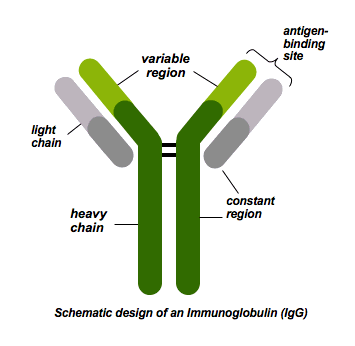
\includegraphics{../Images/schematics_antibody.png}